\section{Results}
\label{section:discussion&results:experiment-results}

This section presents the results acquired from executing the experiments defined in \Cref{section:Results:ExperimentalPlan}.
Results are presented with average values of error metrics per dataset, as well as box-plots of error metrics,
and t-test results between the explored models.

All results for each of the experiments can be found in \Cref{appendix:all-results}.

% Dataset 1
\subsection{Dataset 1}
% Results
\import{./tables/results/dataset_1}{Average-metric-dataset-1.tex}
% T-test smapev
% T-test smapev
\import{./tables/results/ttest}{ttest-p-values-lstm-experiments-sMAPE.tex}
\import{./tables/results/ttest}{ttest-p-values-main-experiments-sMAPE.tex}
% \import{./tables/results/ttest}{ttest-p-values-lstm-experiments-MASE.tex}

\begin{figure}[h!]
  \centering
  \label{fig:results:boxplot-dataset-1}
  \caption{Boxplot of predictions made on dataset 1}
  \begin{subfigure}[b]{0.49\textwidth}
    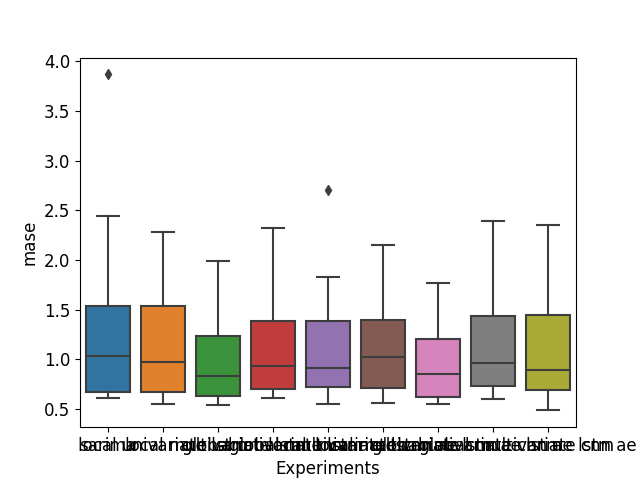
\includegraphics[width=\textwidth]{./figs/results/boxplot/mase-dataset_1.png}
    \hfill
    \caption{MASE boxplot of predictions made on dataset 1}
    \label{fig:results:boxplot-mase-dataset-1-mase}
  \end{subfigure}
  \begin{subfigure}[b]{0.49\textwidth}
    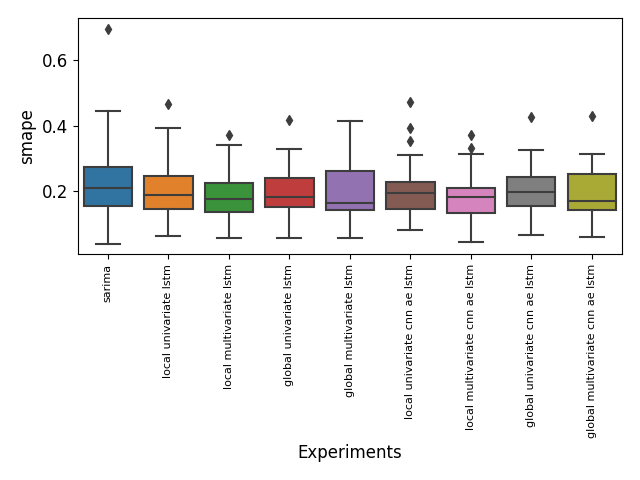
\includegraphics[width=\textwidth]{./figs/results/boxplot/smape-dataset_1.png}
    \hfill
    \caption{sMAPE boxplot of predictions made on dataset 1}
    \label{fig:results:boxplot-mase-dataset-1-smape}

  \end{subfigure}
\end{figure}
% \begin{figure}[h!]
%   \centering
%   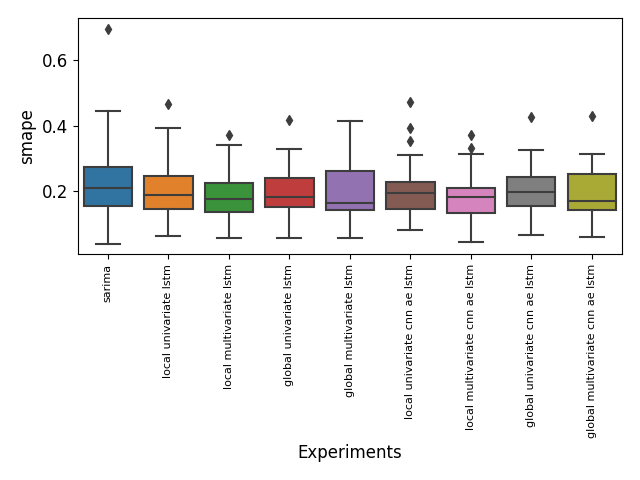
\includegraphics[width=\textwidth]{./figs/results/boxplot/smape-dataset_1.png}
%   \hfill
%   \caption{sMAPE boxplot of predictions made on dataset 1}
%   \label{fig:results:boxplot-mase-dataset-1-smape}
% \end{figure}

\Cref{table:Average-metric-dataset-1} shows the mean metrics across
all the time series in dataset 1.
\Cref{table:ttest-p-values-lstm-experiments-sMAPE} show the p-values
for every LSTM structure compared with the local univariate LSTM.
\Cref{table:ttest-p-values-main-experiments-sMAPE} show the p-values
comparing the sMAPE results between the LSTM and the CNN-AE-LSTM for each
model structure.
The poorest performing model across the board
is SARIMA, with a MASE of $1.294$, sMAPE of $0.239$ and 7-day MASE of $1.063$.
All the different LSTM structures and hybrid methods outperformed SARIMA,
as seen in \Cref{fig:results:boxplot-mase-dataset-1-smape}.

The multivariate models outperformed all their retrospective univariate counter partners.
The global univariate LSTM outperforms the local univariate on both MASE and sMAPE, though not statistically significant,
but this results is not reproduced for the multivariate models, or the CNN-AE-LSTM models.

All the model structures performs slightly better with our proposed CNN-AE-LSTM method on dataset 1, except for
the global univariate CNN-AE-LSTM.

The most consistent models with the least amount of variance are the multivariate models.
The local multivariate CNN-AE-LSTM and the local multivariate LSTM were the only two models
who beat the naive 7-day prediction. The best performing model is the local multivariate CNN-AE-LSTM.


% Is this needed? What does this tell us? Is this something we comment on later?
\iffalse
The mean MASE dataset across all models on dataset 1 is $0.971$,
the mean sMAPE is $0.2034$,
and the mean MASE 7-day is $0.9976$.
\fi






\subsection{Dataset 2}
% Dataset 2

\begin{samepage}
  \import{./tables/results/dataset_2}{Average-metric-dataset-2.tex}
  \begin{figure}[ht!]
    \caption{Boxplot of predictions made on dataset 2}
    \centering
    \begin{subfigure}[b]{0.49\textwidth}
      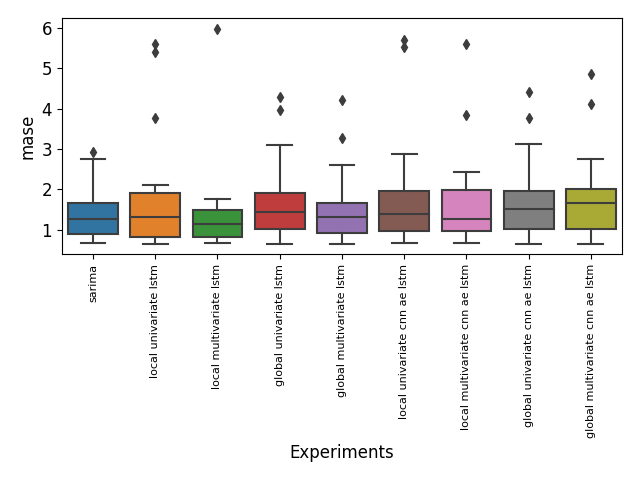
\includegraphics[width=\textwidth]{./figs/results/boxplot/mase-dataset_2.png}
      \hfill
      \caption{Boxplot of the MASE metrics}
      \label{fig:results:boxplot-mase-dataset-2-mase}
    \end{subfigure}
    \begin{subfigure}[b]{0.49\textwidth}
      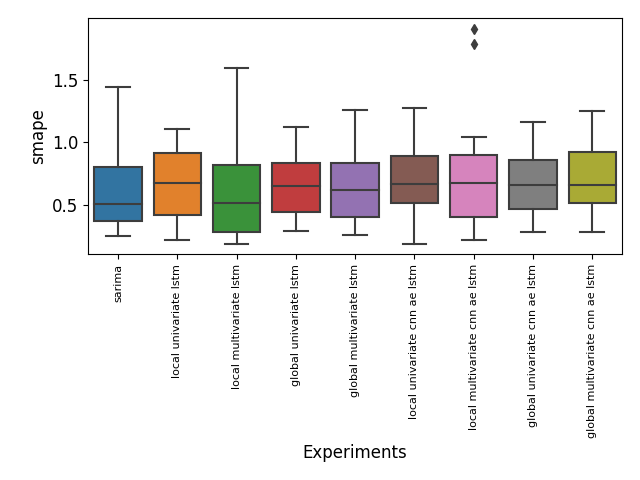
\includegraphics[width=\textwidth]{./figs/results/boxplot/smape-dataset_2.png}
      \hfill
      \caption{Boxplot of the sMAPE metrics}
      \label{fig:results:boxplot-mase-dataset-2-smape}
    \end{subfigure}
    \label{fig:results:boxplot-dataset-2}
  \end{figure}
\end{samepage}

The results from dataset 2 are shown in \Cref{table:Average-metric-dataset-2},
and visualized in Figure \ref{fig:results:boxplot-dataset-2}. The p-values
are in \Cref{table:ttest-p-values-lstm-experiments-sMAPE} and
\Cref{table:ttest-p-values-main-experiments-sMAPE}.

Compared to dataset 1, dataset 2 proved to be a much more difficult dataset to forecast.
Compared to the neural network models, SARIMA performs better, with a mase of $1.472$, a 7-day MASE of $0.707$ and a smape of $0.633$.
Some of the results from dataset 1 are reproduced on dataset 2. For example, the global univariate LSTM outperforms
the local univariate LSTM. The multivariate models outperform the univariate models.
On dataset 2 however, all the CNN-AE-LSTM methods perform poorly compared to the LSTM models.
The best performing model on dataset 2 is local multivariate LSTM with a mase of $1.377$ a sMAPAE of $0.603$
and $0.697$.


% Is this needed? What does this tell us? Is this something we comment on later?
\iffalse
The mean MASE across dataset 2 is $1.652$,
the mean sMAPE is $0.697$,
and the mean MASE 7-day is  $0.7306$.
\fi





% Dataset 3
\subsection{Dataset 3}
\begin{samepage}
  \import{./tables/results/dataset_seasonal}{Average-metric-dataset-3.tex}
  \begin{figure}[h!]
    \centering
    \caption{Boxplot of predictions made on the seasonal dataset 3}
    \begin{subfigure}[t]{0.49\textwidth}
      \includegraphics[width=\textwidth]{./figs/results/boxplot/mase-dataset_3.png}
      \hfill
      \caption{MASE boxplot. The local multivariate CNN-AE-LSTM performs best,
        while the global multivariate CNN-AE-LSTM performs worst.}
      \label{fig:results:boxplot-mase-dataset-3}

    \end{subfigure}
    \begin{subfigure}[t]{0.49\textwidth}
      \includegraphics[width=\textwidth]{./figs/results/boxplot/smape-dataset_3.png}
      \hfill
      \caption{sMAPE boxplot. The local multivariate CNN-AE-LSTM performs best,
        but with a higher variance than on MASE.
        The global multivariate CNN-AE-LSTM performs worst.}
      \label{fig:results:boxplot-smape-dataset-3}
    \end{subfigure}
    \label{fig:results:boxplot-dataset-3}
  \end{figure}
\end{samepage}
The results from dataset 3 is in \Cref{table:Average-metric-dataset-3},
and visualized in \Cref{fig:results:boxplot-dataset-3}.
The p-values are in \Cref{table:ttest-p-values-lstm-experiments-sMAPE} and
\Cref{table:ttest-p-values-main-experiments-sMAPE}.
On dataset 3 SARIMA, again, outperforms the purely local univariate LSTM baseline.
Many of the same patterns repeats on dataset 3 as with dataset 1 and 2, multivariate beats univariate,
global unviariate beats local univariate.
On dataset 3 it seems that the CNN-AE-LSTMs outperform the LSTMs once again, except for the
best perfoming model, which is the local multivariate LSTM.


% Is this needed? What does this tell us? Is this something we comment on later?
\iffalse
% These values are not updated. It should be updated if we consider using it in the text.
The mean MASE for dataset 3 is $1.957$,
the mean sMAPE data set 3 is $0.431$,
and the mean MASE 7-day is $1.111$.
\fi







% Globale modeller er dårligere på mase 7 bortsett fra.
% All results tables

\subsection{Model Comparisons Across Datasets}
Due to the low sample size of the available datasets,
proving the statistical significance of model performance proves to be a difficult task.
However, aggregating the results across the 3 datasets will increase the sample size of the predictions.
This will, in turn, improve the basis for doing statistical tests on the model predictions. 

%Our results suffer from low sample size and high variance, so it isn't easy
%to prove anything statistically. Aggregating the results across the datasets
%increases our sample size, improving the statistical tests.

\import{./tables/results/}{Average-metric-all-datasets.tex}
\import{./tables/results/ttest}{ttest-p-values-lstm-experiments-sMAPE-all-dataset.tex}
\begin{figure}
  \begin{subfigure}[b]{0.49\textwidth}
    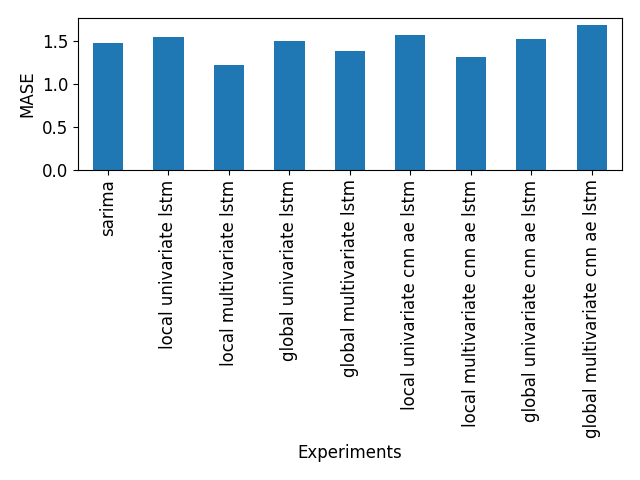
\includegraphics[width=\textwidth]{./figs/results/barplot/MASE-all-dataset.png}
    \hfill
    \caption{Boxplot of predictions made on seasonal dataset}
    % \label{fig:results:boxplot-mase-dataset-3}
  \end{subfigure}
  \begin{subfigure}[b]{0.49\textwidth}
    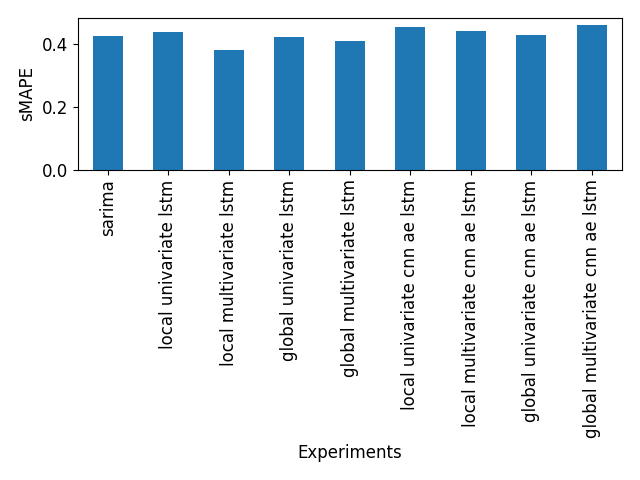
\includegraphics[width=\textwidth]{./figs/results/barplot/sMAPE-all-dataset.png}
    \hfill
    \caption{Boxplot of predictions made on seasonal dataset}
    % \label{fig:results:boxplot-mase-dataset-3}

  \end{subfigure}
\end{figure}

\subsubsection{LSTM models}
% \subsubsection{Local Versus Global}
The global univariate LSTM model improves prediction error over the local univariate model
by $2.4\%$ with the sMAPE metric.
Additionally, applying the t-test implies that this difference in metric is not significant,
with a p-value of $0.712$.
However, in order to measure the difference in the models we compare the models across all of the datasets.
By aggregating the prediction metrics, as shown in \Cref*{table:Average-metric-all-datasets},
we achieve an improvement of $4.43\%$ instead. Additionally, the p-value from the statistical t-test
has a significant decrease in value to $0.362$, as shown in \Cref*{table:ttest-p-values-lstm-experiments-sMAPE-all-dataset}.
Although this is still not enough for the t-test to indicate a statistically significant difference,
we are able to see a clear trend indicating that the global univariate model is an improvement compared to the local univariate model.

%From dataset 1, the global univariate LSTM improves the local univariate
%LSTM by $2.4\%$, however, can be random with a p-value of $0.712$.
%When we compare both model structures across all the datasets,
%as shown in \Cref{table:Average-metric-all-datasets},
%our global model improves by $4.43\%$ relative to the local model,
%and our p-value falls to $0.362$, as shown in \Cref{table:ttest-p-values-lstm-experiments-sMAPE-all-dataset}.
%Even though this is not low enough
%to be below our threshold value of $0.05$, does show a promising trend.





% \subsubsection{Univariate Versus Multivariate}
The local multivariate LSTM shows a big improvement over the local univariate LSTM.
On average, the performance of the model reduces predictive error by $13.74\%$ using the sMAPE error metric.
Additionally, the p-value of the t-test shows a value of $0.039$, thus implying a significant difference in predictions.



% \subsubsection{Global Multivariate Versus Global Univariate}
The global multivariate LSTM model improves predictive error by $4.2\%$ over the local univariate LSTM model,
and $3.1\%$ over the global univariate model.
In addition to outperforming the local univariate baseline, the global multivariate model also outperformed the global univariate model.
However, the t-tests for the model are all above the threshold of $0.05$ compared to both models.
The global multivariate model is not able to outperform the local multivariate model,
with a predictive error of $7.33\%$ worse than the local multivariate model.






\subsection{Hybrid model compare results}
\label{section:discussion&results:experiment-results:CNN-AE-LSTM}
The hybrid methods can be compared with the LSTM baseline methods.
The experiment results used in this section comes from results tables
\Cref*{table:Average-metric-dataset-1}, \Cref*{table:Average-metric-dataset-2}, \Cref*{table:Average-metric-dataset-3},
as well as the tables for t-test values, \Cref*{table:ttest-p-values-main-experiments-sMAPE}.


\subsubsection{Local univariate}
% Local univariate CNN-AE-LSTM
\label{section:discussion&results:experiment-results:CNN-AE-LSTM:Local-Univariate}
The local univariate LSTM and the local univariate convolutional autoencoder and LSTM are one of the model-configurations
that offer rather similar results across datasets.
While the hybrid model performance is more or less equal, predictions made on datasets 2 and 3 vary a bit more
with the basic LSTM model performs 4.6\% and 1.25\% better on average.
However, in addition to these similarities in average performance, the T-test conducted on the experiments reveals the same outcome.
The t-test Resultsults shown in \Cref{table:ttest-p-values-main-experiments-sMAPE} infer that the predictions made by the two local univariate models
are from the same group, and there is no significant difference in their distribution.



% TODO: Improve language
\subsubsection{Global univariate}
\label{section:discussion&results:experiment-results:CNN-AE-LSTM:Global-Univariate}
% Global univariate
The global univariate CNN-AE-LSTM model is, on average, an improvement over the local univariate CNN-AE-LSTM model.
The model outperforms the local univariate model on datasets 2 and 3, but not on dataset 1.
However, the global model performs better than the local model for all datasets with
a $5.5\%$ lower sMAPE error metric.
The global univaraite CNN-AE-LSTM model is not able to outperforme the global univariate LSTM model.
The global univariate LSTM model generally performed better than the hybrid model.
Evaluating the difference with the t-test, it is also clear that the difference is significant.

% Dataset 1 is significantly worse (Can se this fom the individual dataset performances, where it is more or less always worse, and t-test says significanse)
% Dataset 2 is significantly different / worse (LSTM is generaly better, although there are more differences. Sometimes hybrid is better, but mostly, LSTM is best)
% Dataset 3 offers no significant difference. This could be contributed to the low sample size (only 8 time series)
Although the average metrics performance between the hybrid model and the LSTM model on dataset 1 is only a little under 4\%,
there is still quite a difference.
By evaluating the metrics of each prediction in the dataset, as well as using the significance test results from the t-test,
it is clear that the global univariate LSTM model is significantly better than the global univariate convolutional autoencoder and LSTM for dataset 1.
For dataset 2 the difference is not as prominent as with dataset 1, but also here, there is a significant difference in predictions.
Only with dataset 3, where the hybrid model performs better than the LSTM model on average as a global univariate model,
the t-test signals that there are no significant differences between the two predictions.
However, it is unclear if this is due to the dataset or if this has to do with the low sample size compared to dataset 1 and dataset 2.




\subsubsection{Local multivariate}
\label{section:discussion&results:experiment-results:CNN-AE-LSTM:Local-Multivariate}
% Local multivariate
The local multivariate CNN-AE-LSTM model serves a slight improvement to predictions for datasets 1 and 3,
although there are no clear improvements to predictions.
On average, dataset 1 is improved with $1.1\%$ and dataset 3 is improved with $1.4\%$ for the sMAPE error metric.
The t-test applied to the predictions supports this assumption as there are no significant
differences between the predictions made with the local multivariate model.

However, the results are quite different for dataset 2.
The CNN-AE-LSTM model increases the sMAPE error metric with $23\%$ over the local multivariate LSTM model, thus decreasing performance significantly.
This is also supported by the t-test conducted, implying a significant difference in prediction sMAPE errors.




\subsubsection{Global multivariate}
\label{section:discussion&results:experiment-results:CNN-AE-LSTM:Global-Multivariate}
% Global Multivariate
On dataset 1 the global multivariate hybrid model performs on average 2\% better than the global multivariate LSTM model. However, there is not a significant difference.
This is supported by the results from the t-test, which implies there is no significance in the difference in predictions.
While there was a significant difference between the models using a global univariate model, the difference in performance was not high.


Unfortunately, the same does not apply to dataset 2 and dataset 3.
While the hybrid model, on average, perform about 9.5\% worse on dataset 2, it also performs about 41.9\% worse on dataset 3.
Applying the student t-test to the predictions also supports the notion of the global multivariate model decreasing performance for the
convolutional autoencoder and LSTM.
Both predictions for dataset 2 and dataset 3 are well within the confidence interval of the t-test,
thus implying a significant difference between the predictions for datasets 2 and 3.



